\section{Time-Dependent Schrödinger Equation}

\begin{frame}{Approach to the Schrödinger equation}
    Moving in the quantum realm, our next goal is to approximate the solution of a \textbf{1D time-dependent \textcolor{BrickRed}{Schrödinger equation}}:

    \begin{equation*}
        \fcolorbox{BrickRed}{white}{\text{$\displaystyle i\hbar\frac{\partial\psi}{\partial t}=-\frac{\hbar^2}{2m}\frac{\partial^2\psi}{\partial x^2}+V(x)\psi(x,t)$}}
    \end{equation*}

    \pause

    \begin{equation*}
        \Big\Downarrow
    \end{equation*}

    \small

    \begin{equation*}
        \underbrace{i\hbar\sum_{j=1}^N\frac{d\psi_j}{dt}\int_{-L}^L\phi_j\phi_idx}_{i\hbar M\frac{d\boldsymbol{\psi}}{dt}}=\underbrace{\frac{\hbar^2}{2m}\sum_{j=1}^N\psi_j\int_{-L}^L\frac{\partial\phi_j}{\partial x}\frac{\partial\phi_i}{\partial x}dx}_{\frac{\hbar^2}{2m}A\boldsymbol{\psi}}+\sum_{j=1}^N\psi_j\int_{-L}^LV\phi_j\phi_idx
    \end{equation*}

    \normalsize
\end{frame}

\begin{frame}{Potential matrix}
    In the equation it appears a \underline{linear term}.

    \pause
    
    We must then introduce a new matrix, that can be called \textcolor{BrickRed}{\textbf{potential matrix}}, which is nothing different than a \textbf{weighted mass matrix}:

    \begin{equation*}
        V:V_{i,j}=\int_\Omega V(x)\phi_j(x)\phi_i(x)dx
    \end{equation*}

    \pause

    \begin{equation*}
        \Big\Downarrow
    \end{equation*}

    \begin{equation*}
        i\hbar M\frac{d\boldsymbol{\psi}}{dt}=\frac{\hbar^2}{2m}A\boldsymbol{\psi}+V\boldsymbol{\psi}
    \end{equation*}

    \pause

    \begin{equation*}
        \Big\Downarrow
    \end{equation*}

    \begin{equation*}
        \fcolorbox{BrickRed}{white}{\text{$\displaystyle M\frac{d\boldsymbol{\psi}}{dt}=-\frac{i}{\hbar}\left(\frac{\hbar^2}{2m}A+V\right)\boldsymbol{\psi}$}}
    \end{equation*}
\end{frame}

\begin{frame}{Application of the Cranck-Nicholson method}
    In this case, the PDE is of \underline{first order} in time.

    \pause

    The most suitable method to use is the \textcolor{BrickRed}{\textbf{Crank-Nicholson}} scheme:

    \begin{equation*}
        M\frac{\boldsymbol{\psi}^{(n+1)}-\boldsymbol{\psi}^{(n)}}{\Delta t}=-\frac{i}{2\hbar}\left(\frac{\hbar^2}{2m}A+V\right)\boldsymbol{\psi}^{(n+1)}-\frac{i}{2\hbar}\left(\frac{\hbar^2}{2m}A+V\right)\boldsymbol{\psi}^{(n)}
    \end{equation*}

    \pause

    \begin{equation*}
        \Big\Downarrow
    \end{equation*}

    \begin{equation*}
        \fcolorbox{BrickRed}{white}{\text{$\displaystyle\left[M+\frac{i\Delta t}{2\hbar}\left(\frac{\hbar^2}{2m}A+V\right)\right]\boldsymbol{\psi}^{(n+1)}=\left[M-\frac{i\Delta t}{2\hbar}\left(\frac{\hbar^2}{2m}A+V\right)\right]\boldsymbol{\psi}^{(n)}$}}
    \end{equation*}
\end{frame}

\begin{frame}{How to handle imaginary part}
    The imaginary unit implies that the wavefunction is \underline{complex-valued}.

    \pause

    In order to work with standard real-valued FEM solvers, we apply a \textcolor{BrickRed}{\textbf{real-imaginary splitting}}:

    \begin{equation*}
        \boldsymbol{\psi}^{(i)}=\boldsymbol{u}^{(i)}+i\boldsymbol{w}^{(i)}
    \end{equation*}

    \pause

    Setting $\alpha=\frac{\Delta t}{2\hbar}$ and $H=\frac{\hbar^2}{2m}A+V$:

    \begin{equation*}
        \left(M+i\alpha H\right)\left(\boldsymbol{u}^{(n+1)}+i\boldsymbol{w}^{(n+1)}\right)=\left(M-i\alpha H\right)\left(\boldsymbol{u}^{(n)}+i\boldsymbol{w}^{(n)}\right)
    \end{equation*}

    \pause

    \begin{equation*}
        \Big\Downarrow
    \end{equation*}

    \begin{equation*}
        \begin{cases}
            M\boldsymbol{u}^{(n+1)}-\alpha H\boldsymbol{w}^{(n+1)}=M\boldsymbol{u}^{(n)}+\alpha H\boldsymbol{w}^{(n)}\\
            \alpha H\boldsymbol{u}^{(n+1)}+M\boldsymbol{w}^{(n+1)}=-\alpha H\boldsymbol{u}^{(n)}+M\boldsymbol{w}^{(n)}
        \end{cases}
    \end{equation*}
\end{frame}

\begin{frame}{Block matrix formulation}
    Concatenating real and imaginary components in a \underline{\textit{single} vector}, the final expression is

    \begin{equation*}
        \fcolorbox{BrickRed}{white}{\text{$\displaystyle\begin{pmatrix}
            M & -\alpha H\\
            \alpha H & M
        \end{pmatrix}
        \begin{pmatrix}
            \boldsymbol{u}^{(n+1)}\\
            \boldsymbol{w}^{(n+1)}
        \end{pmatrix}
        =
        \begin{pmatrix}
            M & \alpha H\\
            -\alpha H & M
        \end{pmatrix}
        \begin{pmatrix}
            \boldsymbol{u}^{(n)}\\
            \boldsymbol{w}^{(n)}
        \end{pmatrix}$}}
    \end{equation*}

    \vfill

    \normalsize

    \begin{center}
        As before, the problem is recast as a \textbf{linear system of equations}.
   \end{center}

    \vfill
\end{frame}

\subsection{Free particle}

\begin{frame}{Free particle scenario}
    If $V(x)=0$, the solution of the Schrödinger equation describes a system called \textcolor{BrickRed}{\textbf{free particle}}.

    \pause

    \vfill

    A \textbf{gaussian} $\mathcal{G}\left(x|x_0,\sigma_0\right)$ can be chosen as \textit{initial wave packet}:

    \begin{equation*}
        \psi(x,0)=\left(\pi\sigma_0^2\right)^{-\frac{1}{4}}e^{-\frac{\left(x-x_0\right)^2}{2\sigma_0^2}+ik_0x}
    \end{equation*}

    We know the analytical solution of the equation:

    \begin{equation*}
        \fcolorbox{BrickRed}{white}{\text{$\displaystyle\psi(x,t)=\frac{1}{\sigma_t\sqrt{\pi}}e^{-\frac{\left(x-x_0-\frac{\hbar k_0}{m}t\right)^2}{\sigma_t^2}} \ \ \ \ \text{where} \ \sigma_t=\sigma_0\sqrt{1+\left(\frac{\hbar t}{m\sigma_0^2}\right)^2}$}}
    \end{equation*}
\end{frame}

\begin{frame}{Numerical simulation}
    Numerical simulation using FEM confirms the theoretical predictions.

    \begin{figure}[H]
        \centering
        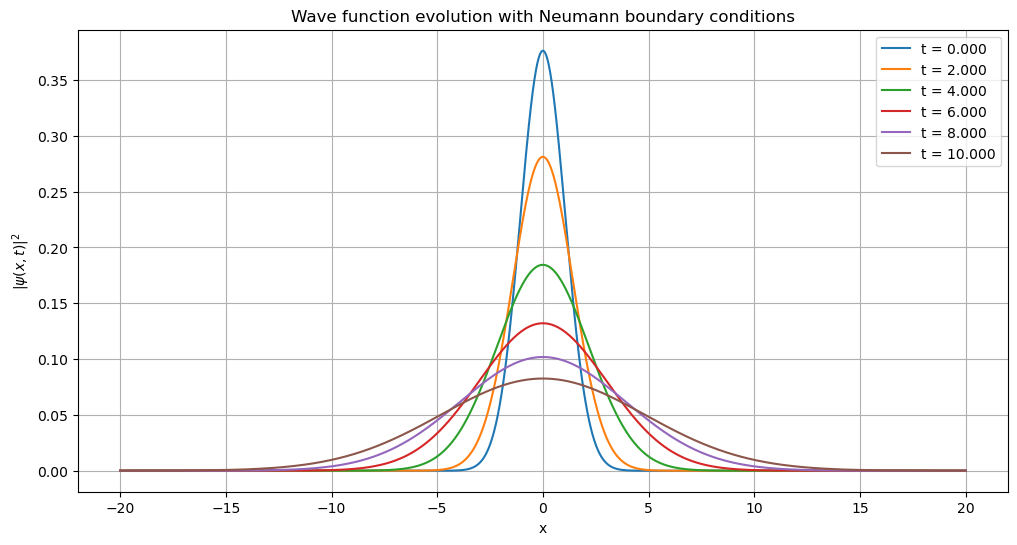
\includegraphics[width=\textwidth]{Immagini/plot-schrodinger-free-particle.png}
    \end{figure}
\end{frame}

\begin{frame}{Ballistic spreading}
    The numerical $\sigma$ follows the same \textbf{ballistic behaviour} up until the time when the wavefunction \underline{reaches the boundary}.

    \begin{equation*}
        \sigma(t)\propto\frac{t}{\sigma_0} \ \longrightarrow \ \text{Bigger $\sigma_0$, slower spreading}
    \end{equation*}

    \pause

    \vfill

    \visible<2>{\begin{minipage}{0.31\textwidth}
        \begin{center}
            $\sigma_0=0.10$
        \end{center}
        \vspace{-0.25cm}
        \begin{figure}
            \centering
            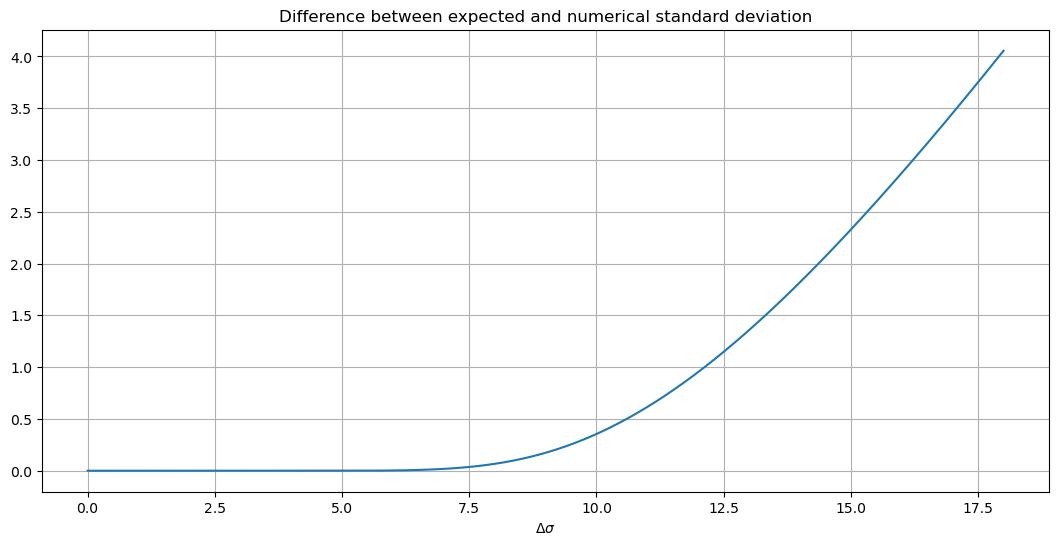
\includegraphics[width=\textwidth]{Immagini/plot-sigma-diff-1.png}
        \end{figure}
    \end{minipage}
    \hfill
    \begin{minipage}{0.31\textwidth}
        \begin{center}
            $\sigma_0=0.15$
        \end{center}
        \vspace{-0.25cm}
        \begin{figure}
            \centering
            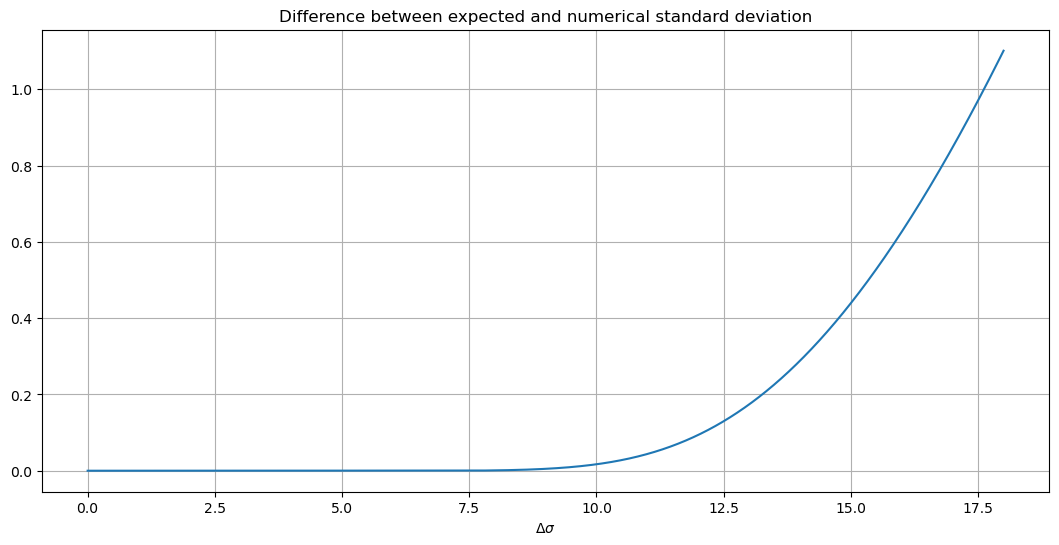
\includegraphics[width=\textwidth]{Immagini/plot-sigma-diff-1,5.png}
        \end{figure}
    \end{minipage}
    \hfill
    \begin{minipage}{0.31\textwidth}
        \begin{center}
            $\sigma_0=0.20$
        \end{center}
        \vspace{-0.25cm}
        \begin{figure}
            \centering
            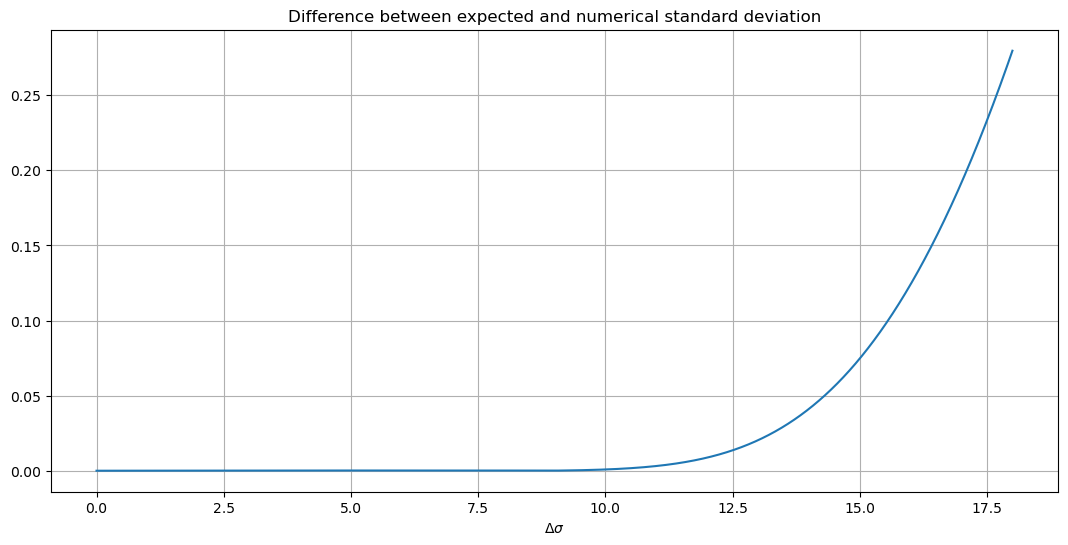
\includegraphics[width=\textwidth]{Immagini/plot-sigma-diff-2.png}
        \end{figure}
    \end{minipage}

    \vspace{-0.15cm}

    \begin{figure}[H]
        \centering
        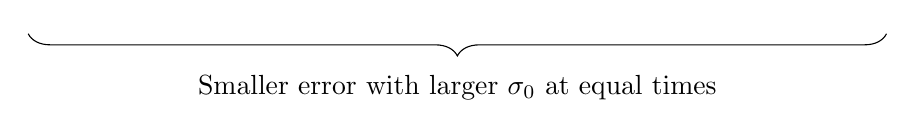
\begin{tikzpicture}
            \draw[decorate, decoration={brace, amplitude=8pt, raise=2pt}] (5.45,0) -- (-5.45,0);

            \node at (0,-0.75) () {Smaller error with larger $\sigma_0$ at equal times};
        \end{tikzpicture}
    \end{figure}}
\end{frame}

\subsection{Periodic potential}

\begin{frame}{Kronig-Penney model}
    The introduction of a \textbf{periodic potential} leads to what is called a \textcolor{BrickRed}{\textbf{Kronig-Penney-like model}}, which is used to describe electrons in a \underline{crystal lattice}.

    \pause

    \begin{center}
      \begin{framed}
        \textcolor{BrickRed}{\textbf{Bloch's theorem}} states that solutions to the Schrödinger equation in a \underline{periodic potential} can be expressed as \textit{plane waves} modulated by \textit{periodic functions} $u(x)$ with the same periodicity as the crystal:

        \begin{equation*}
            \psi(x)=e^{ikx}u(x)
        \end{equation*}
      \end{framed}
   \end{center}
\end{frame}

\begin{frame}{Bloch waves}
    A periodic potential $V(x)=V_0\cos\left(\frac{2\pi}{a}x\right)$ couples plane waves which differ of multiples of $\frac{2\pi}{a}$, and the resulting superpositions form the \textcolor{BrickRed}{\textbf{Bloch waves}}.

    \vspace{-0.15cm}

    \begin{equation*}
        \text{Projection onto periodic plane waves}
    \end{equation*}

    \vspace{-0.3cm}

    \begin{equation*}
        \Big\downarrow
    \end{equation*}

    \vspace{-0.25cm}

    \begin{equation*}
        \text{Formation of \textbf{lattice harmonics}}
    \end{equation*}

    \vfill

    \begin{minipage}{0.32\textwidth}
        \begin{center}
            $a=1.0$
        \end{center}
        \vspace{-0.25cm}
        \begin{figure}
            \centering
            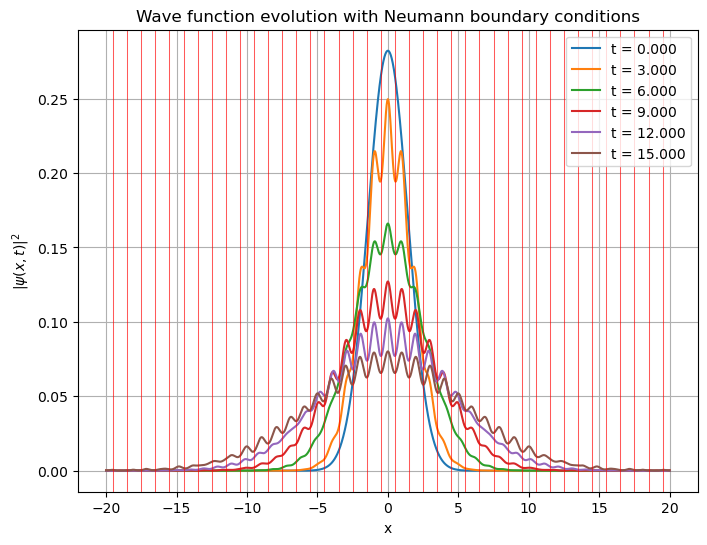
\includegraphics[width=\textwidth]{Immagini/plot-periodic-potential-a-1.png}
        \end{figure}
    \end{minipage}
    \hfill
    \begin{minipage}{0.32\textwidth}
        \begin{center}
            $a=1.5$
        \end{center}
        \vspace{-0.25cm}
        \begin{figure}
            \centering
            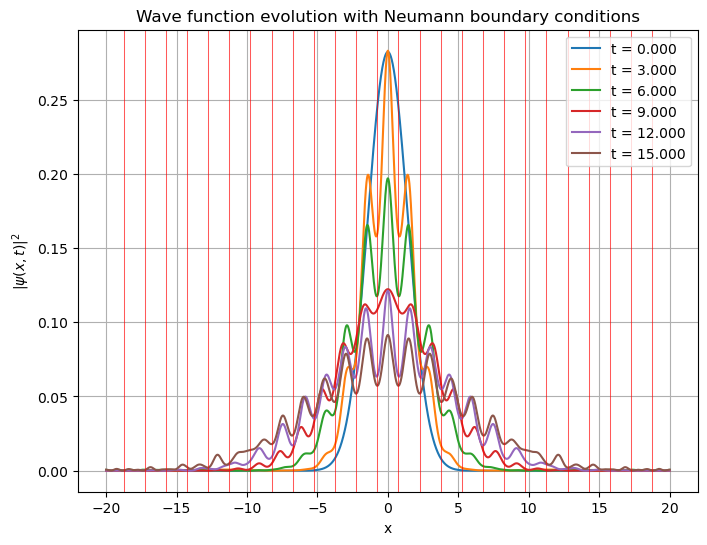
\includegraphics[width=\textwidth]{Immagini/plot-periodic-potential-a-1,5.png}
        \end{figure}
    \end{minipage}
    \hfill
    \begin{minipage}{0.32\textwidth}
        \begin{center}
            $a=2.0$
        \end{center}
        \vspace{-0.25cm}
        \begin{figure}
            \centering
            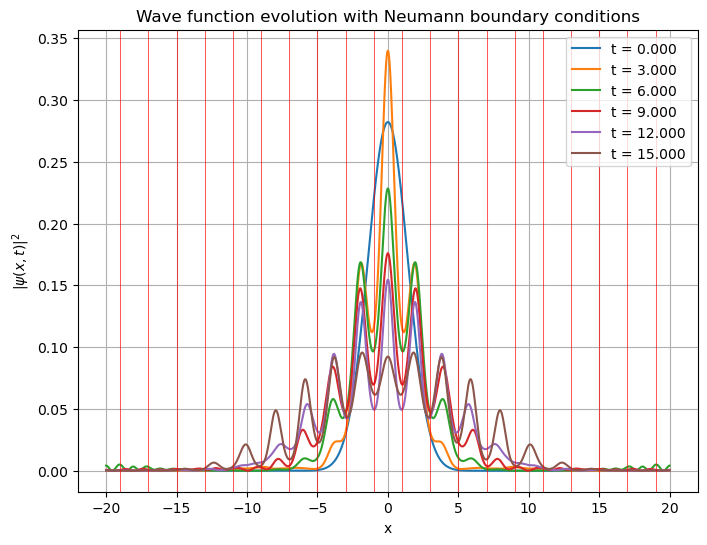
\includegraphics[width=\textwidth]{Immagini/plot-periodic-potential-a-2.png}
        \end{figure}
    \end{minipage}
\end{frame}

\begin{frame}{Effective mass}
    \small

    With the periodic potential, the allowed energies are \underline{no longer continuous}, but split into separate \textbf{bands}, each associated with different values of the \textit{crystal momentum} $k$.

    \vfill

    \pause

    \footnotesize

    Taylor expansion around $k_0$:

    \begin{equation*}
        E(k)=E\left(k_0\right)+\frac{dE}{dk}\bigg|_{k_0}\left(k-k_0\right)+\frac{1}{2}\frac{d^2E}{dk^2}\bigg|_{k_0}\left(k-k_0\right)^2+\dots
    \end{equation*}

    \pause

    In the lowest bound, $k_0=0$ is the \textit{minimum}:

    \begin{equation*}
        E(k)\simeq E_0+\frac{1}{2}\frac{d^2E}{dk^2}\bigg|_{k=0}k^2
    \end{equation*}

    \pause

    Comparing with the energy of a free particle, an \textcolor{BrickRed}{\textbf{effective mass}} can be found:

    \begin{equation*}
        E(k)=E_0+\frac{\hbar^2k^2}{2m^*} \ \Longrightarrow \ \fcolorbox{BrickRed}{white}{\text{$\displaystyle m^*=\hbar^2\left(\frac{d^2E}{dk^2}\bigg|_{k=0}\right)^{-1}$}}
    \end{equation*}

    \normalsize
\end{frame}

\begin{frame}{Sub-ballistic spreading}
    \small

    Around the \textit{minimum of a band}, a quantum system in a periodic lattice behaves like a free particle with an effective mass $m^*$.

    \vfill

    Since $\sigma\propto\frac{1}{m}$, a slower spreading is expected for a periodic lattice where $m^*>m$, due to the \textbf{parabolic approximation} of the band energy.

    \vfill

    \begin{figure}[H]
        \centering
        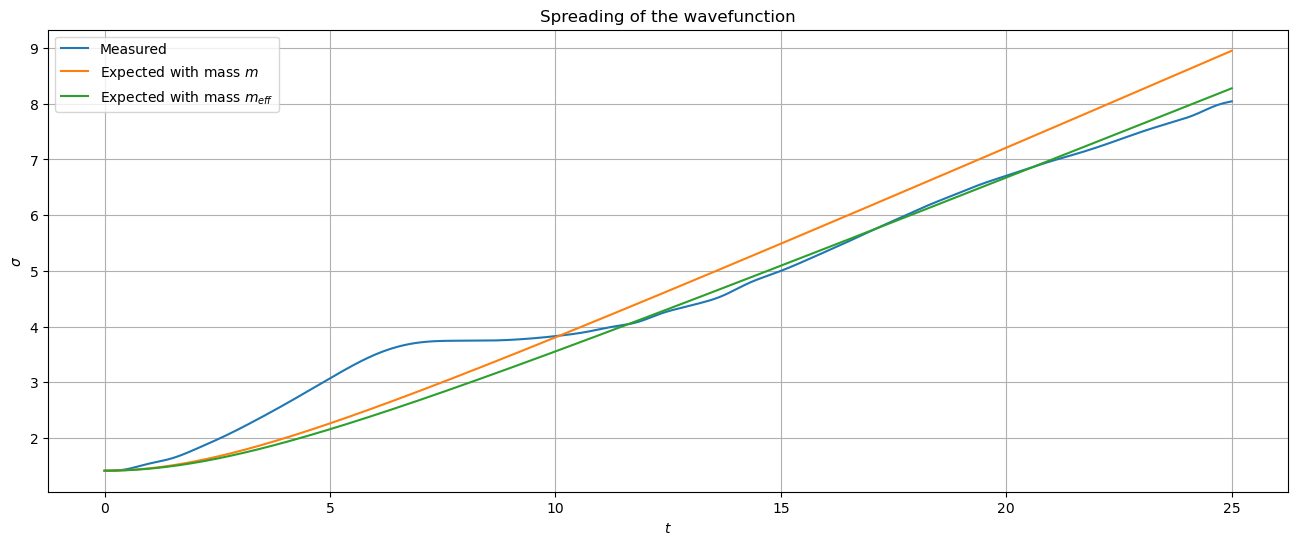
\includegraphics[width=\textwidth]{Immagini/plot-effective-mass.png}
    \end{figure}

    \normalsize
\end{frame}

\subsection{Linear potential}

\begin{frame}{Addition of a linear term}
    The mean value, on the contrary, \underline{does not change}.

    \vfill

    \pause

    In order to induce a \textit{net drift}, we must add a \textbf{linear potential} $V(x)=Fx$.

    \vfill

    \vspace{-0.1cm}

    \visible<2>{\begin{figure}[H]
        \centering
        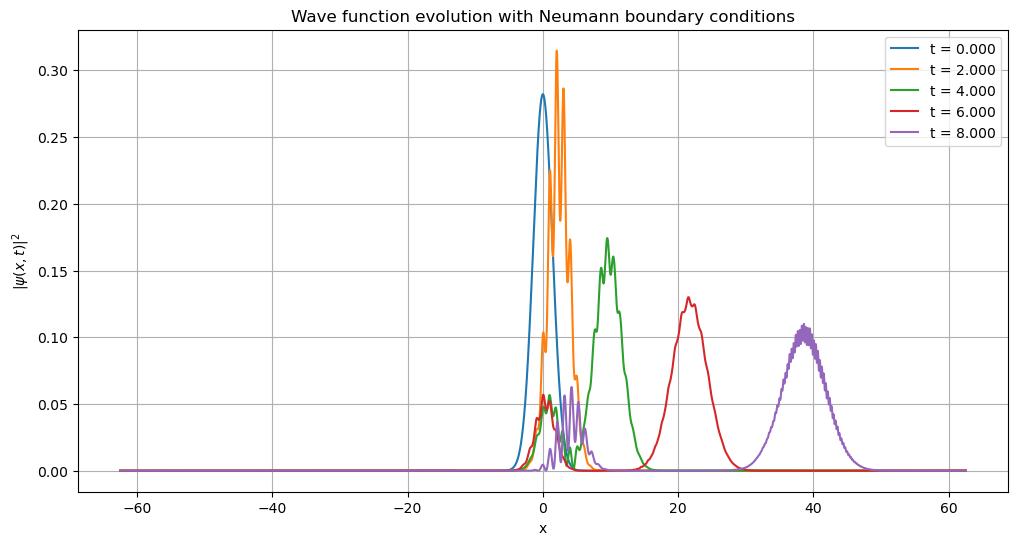
\includegraphics[width=0.87\textwidth]{Immagini/plot-linear-potential.png}
    \end{figure}}

    \vspace{-0.5cm}

    \footnotesize

    \begin{center}
        The plot shows how \underline{dispersion} causes \textbf{interference effects} to gradually \textit{fade}.
    \end{center}

    \normalsize
\end{frame}

\begin{frame}{Average shift}
    \vfill

    \begin{minipage}[c]{0.45\textwidth}
        \begin{figure}
            \centering
            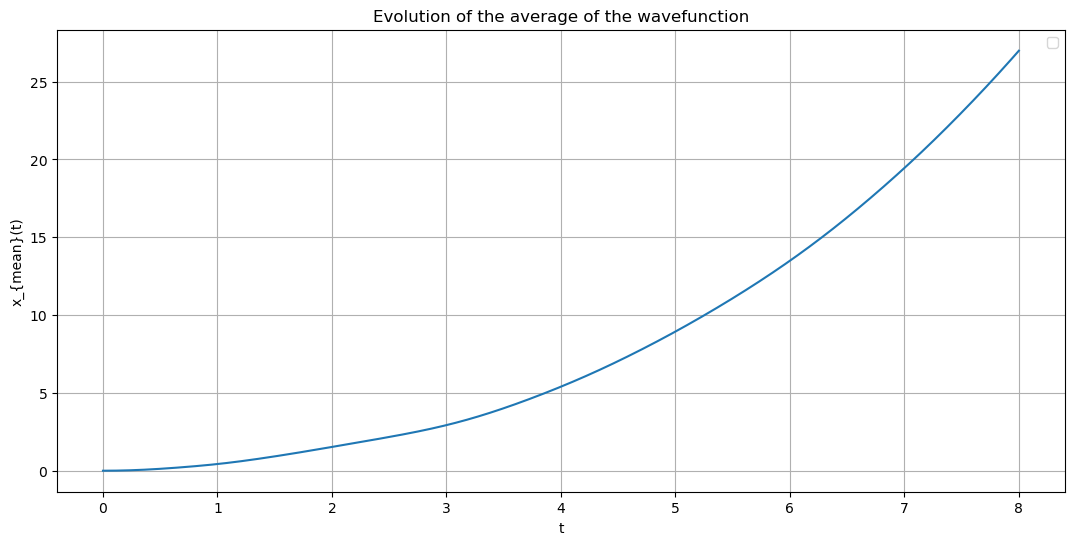
\includegraphics[width=\textwidth]{Immagini/plot-moving-average-1.png}
            \caption*{$V_0=1.00$, $F=1.00$}
        \end{figure}
    \end{minipage}
    \hfill
    \begin{minipage}[c]{0.45\textwidth}
        \begin{figure}
            \centering
            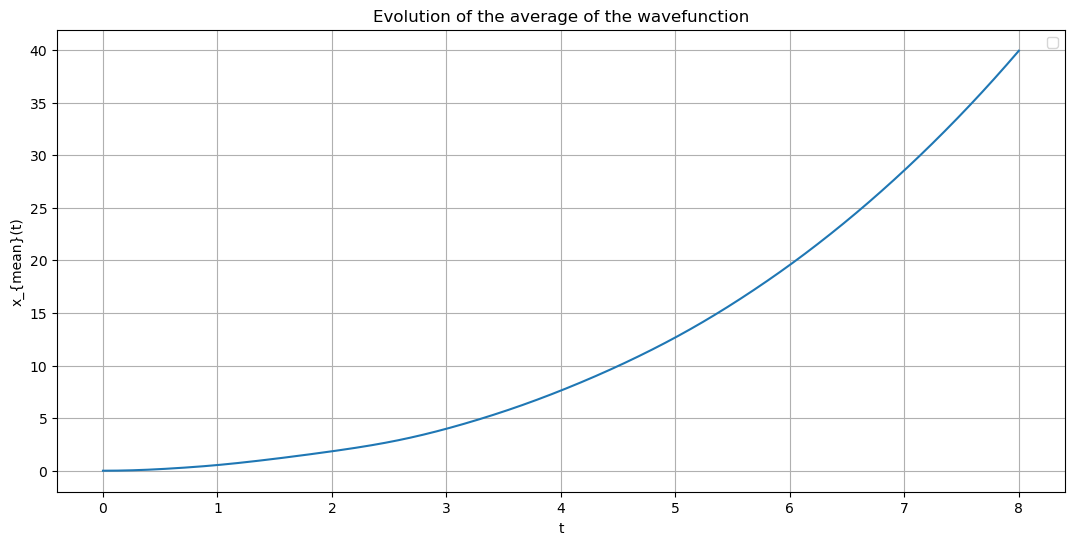
\includegraphics[width=\textwidth]{Immagini/plot-moving-average-1,25.png}
            \caption*{$V_0=1.00$, $F=1.25$}
        \end{figure}
    \end{minipage}

    \vfill

    \begin{minipage}[c]{0.45\textwidth}
        \begin{figure}
            \centering
            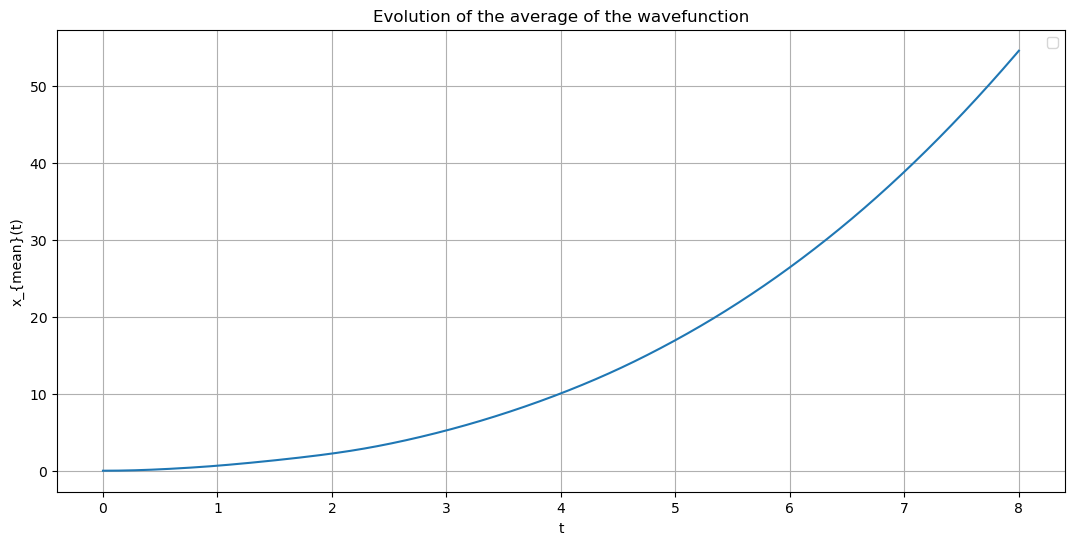
\includegraphics[width=\textwidth]{Immagini/plot-moving-average-1,5.png}
            \caption*{$V_0=1.00$, $F=1.50$}
        \end{figure}
    \end{minipage}
    \hfill
    \begin{minipage}[c]{0.45\textwidth}
        \begin{figure}
            \centering
            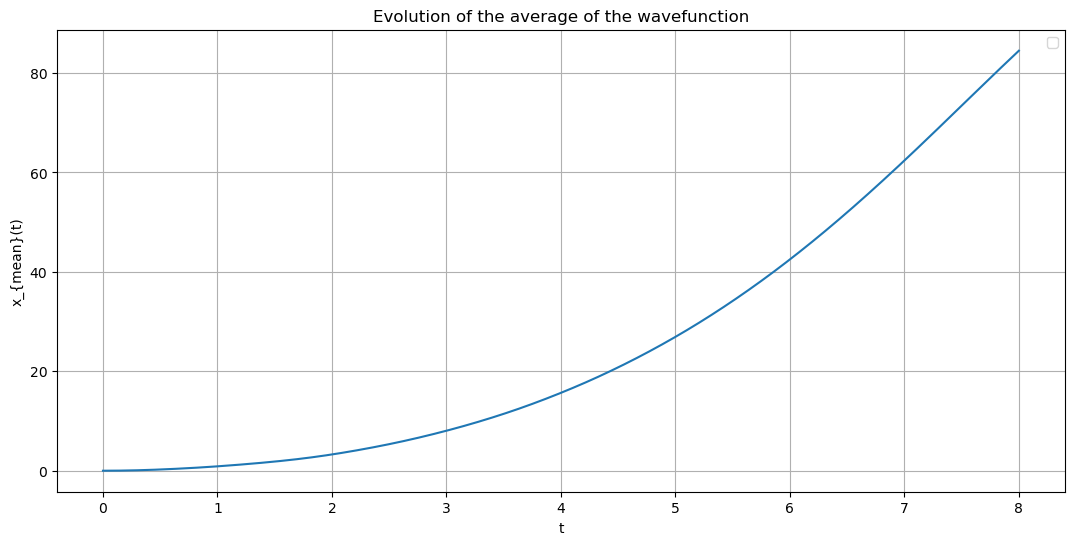
\includegraphics[width=\textwidth]{Immagini/plot-moving-average-2.png}
            \caption*{$V_0=1.00$, $F=2.00$}
        \end{figure}
    \end{minipage}
\end{frame}

\begin{frame}{Conclusions}
    Some final considerations:

    \vfill

    \pause

    \begin{itemize}
        \item FEM provides a suitable approach for \textbf{second-order PDEs}
        \pause
        \item Even though it has been used for very simple domains, in principle it can be applied to very \textbf{complex geometries}
        \pause
        \item To handle time evolution, FEM must be coupled with \textbf{finite difference schemes} or other temporal integration methods
        \pause
        \item The choice of spatial mesh and time step must satisfy some \textbf{stability} and \textbf{accuracy criteria} (like CFL condition or norm conservation)
        \pause
        \item FEM allows easy incorporation of \textbf{boundary conditions}
    \end{itemize}

    \vfill

    \pause

    In summary, our examples show that FEM is a very \textbf{robust} and \textbf{versatile} tool for \underline{spatial discretization}, but time evolution requires \textit{appropriate temporal schemes}.
\end{frame}